%!TEX TS-program = xelatex

% HSE Beamer Theme
% by Danil Fedorovykh
% http://hse.ru/staff/df
%
% Version 2.0 (English)
% January 2022

%%% Set up the free HSE Sans font
%%% https://www.hse.ru/info/brandbook/#font

\documentclass[aspectratio=169]{beamer}

\newbool{russian}
\booltrue{russian} % Uncomment if in Russian
\usepackage{HSE-theme/beamerthemeHSE} % Load HSE theme
\usepackage[no-math]{fontspec}      % fonts loading
\usepackage{caption}
\usepackage{subfigure}
\usepackage{subcaption}
\usepackage{hyperref}
\usepackage[dvipsnames]{xcolor}
\usepackage{ragged2e}
\captionsetup[figure]{labelformat=empty}
\captionsetup[subfigure]{labelformat=empty}
\renewcommand*{\thesubfigure}{(\arabic{subfigure})}
\setsansfont{HSE Sans}
%\graphicspath{{./images/}}
\graphicspath{{/home/llyy/Yandex.Disk/personal/knowledge/general/algorithms_course/repo/algorithms_course/2_sorting_simple/lection/images}}


%%% Информация об авторе и выступлении
\title[Title]{Алгоритмы и структуры данных} 
\subtitle{Лекция 2. Простые сортировки}
\author[Author's name]{Илья Сергеевич Бычков\\ \smallskip \scriptsize \url{ibychkov@hse.ru}}
\institute{НИУ ВШЭ - Нижний Новгород}
\date{\today}


\begin{document}

\frame[plain]{\titlepage}

%%%%%%%%%%%%%%%%%%%%%%%%%%%%%%%%%%%%%%%%%%%%%%%%%%%%%%%%%%%%%%%%%%%%%%%%%%%%%%%%%%%%%%%%%%%%%%%%%%
\begin{frame}[c]
%\frametitle{A first slide}

\begin{center}
\Huge Лекция 2.

\Huge Простые сортировки
\end{center}

\end{frame}

%%%%%%%%%%%%%%%%%%%%%%%%%%%%%%%%%%%%%%%%%%%%%%%%%%%%%%%%%%%%%%%%%%%%%%%%%%%%%%%%%%%%%%%%%%%%%%%%%%
\begin{frame}
\frametitle{Простые сортировки}
\framesubtitle{План лекции}

\begin{enumerate}
  \setcounter{enumi}{-1}
  \item{План лекции}
  \item{\textcolor{blue}{Задача сортировки}}
  \item{Простые квадратичные сортировки}
  \item{Специальные сортировки}
\end{enumerate}
\end{frame}



%%%%%%%%%%%%%%%%%%%%%%%%%%%%%%%%%%%%%%%%%%%%%%%%%%%%%%%%%%%%%%%%%%%%%%%%%%%%%%%%%%%%%%%%%%%%%%%%%%
\begin{frame}
\frametitle{Задача сортировки}
\framesubtitle{Задача сортировки}
\justifying
\textcolor{red}{Задача сортировки} — это одна из основных задач в области алгоритмов и структур данных, которая заключается в упорядочивании набора объектов в соответсвии с заданным критерием (оператором).\newline\newline
Примеры задачи сортировки:
\begin{itemize}
\item{Сортировка списка учеников в алфавитном порядке по фамилии}
\item{Сортировка товаров в интернет-магазине по цене от низкой к высокой}
\item{Сортировка строк в таблице базы данных по дате создания}
\item{Сортировка чисел в массиве по возрастанию}
\item{Сортировка сотрудников компании по их должностям от высших к низшим}
\end{itemize}
\end{frame}

%%%%%%%%%%%%%%%%%%%%%%%%%%%%%%%%%%%%%%%%%%%%%%%%%%%%%%%%%%%%%%%%%%%%%%%%%%%%%%%%%%%%%%%%%%%%%%%%%%
\begin{frame}
\frametitle{Простые сортировки}
\framesubtitle{План лекции}

\begin{enumerate}
  \setcounter{enumi}{-1}
  \item{План лекции}
  \item{Задача сортировки}
  \item{\textcolor{blue}{Простые квадратичные сортировки}}
  \item{Специальные сортировки}
\end{enumerate}
\end{frame}


%%%%%%%%%%%%%%%%%%%%%%%%%%%%%%%%%%%%%%%%%%%%%%%%%%%%%%%%%%%%%%%%%%%%%%%%%%%%%%%%%%%%%%%%%%%%%%%%%%
\begin{frame}
\frametitle{Простые квадратичные сортировки}
\framesubtitle{Общее}
\justifying
Простые квадратичные сортировки имеют следующие общие черты:
\begin{itemize}
\item{основываются только на простом и последовательном сравнении элементов}
\item{последовательно увеличивают текущую отсортированную часть массива добавляя один элемент}
\item{имеют временную сложность $\mathcal {O}(n^2)$ в худшем случае\newline}
\end{itemize}
Простые сортировки:
\begin{itemize}
\item{Сортировка выбором (\textcolor{red}{selection sort})}
\item{Сортировка вставками (\textcolor{red}{insertion sort})}
\item{Сортировка пузырьком (\textcolor{red}{bubble sort})}
\end{itemize}
\end{frame}

%%%%%%%%%%%%%%%%%%%%%%%%%%%%%%%%%%%%%%%%%%%%%%%%%%%%%%%%%%%%%%%%%%%%%%%%%%%%%%%%%%%%%%%%%%%%%%%%%%
\begin{frame}
\frametitle{Простые квадратичные сортировки}
\framesubtitle{Сортировка выбором}
\justifying
\textcolor{red}{Сортировка выбором (selection sort)}\newline\newline
Идея:\newline
Последовательное определение i-го элемента отсортированного массива путем поиска минимума/максимума в оставшейся части (начиная с i).

\begin{figure}
    \captionsetup[subfigure]{labelformat=empty}
    \centering
    \subfigure[{ \scriptsize Строение массива, Источник - \href{	https://www.alphacodingskills.com/algo/selection-sort.php}{alphacodingskills} }]{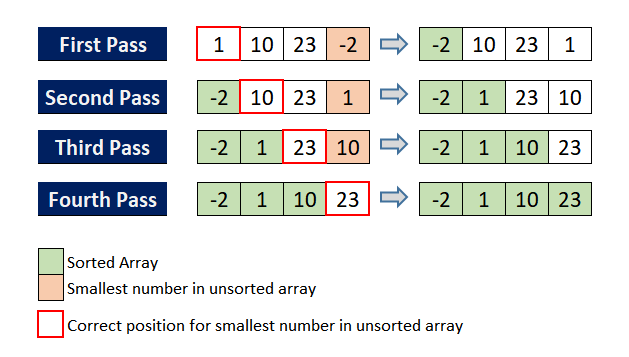
\includegraphics[width=75mm, height=40mm]{selection_sort}} 
\end{figure}
\end{frame}


%%%%%%%%%%%%%%%%%%%%%%%%%%%%%%%%%%%%%%%%%%%%%%%%%%%%%%%%%%%%%%%%%%%%%%%%%%%%%%%%%%%%%%%%%%%%%%%%%%
\begin{frame}
\frametitle{Простые квадратичные сортировки}
\framesubtitle{Сортировка вставками}
\justifying
\small
\textcolor{red}{Сортировка вставками (insertion sort)}\newline\newline
Идея:\newline
Поиск корректной позиции рассматриваемого элемнта в уже отсортированной части массива.

\begin{figure}
    \captionsetup[subfigure]{labelformat=empty}
    \centering
    \subfigure[{ \scriptsize Сортировка вставками, Источник - \href{https://dev.to/conrad96/insertion-sort-28kb}{Dev.to} }]{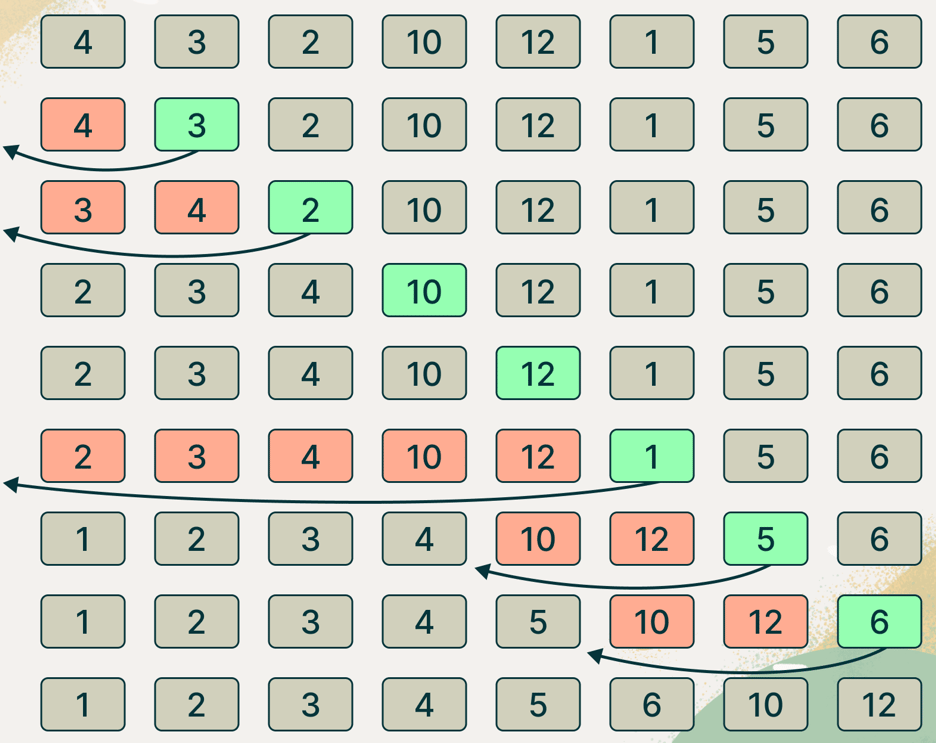
\includegraphics[width=55mm, height=40mm]{insertion_sort}} 
\end{figure}
\end{frame}

%%%%%%%%%%%%%%%%%%%%%%%%%%%%%%%%%%%%%%%%%%%%%%%%%%%%%%%%%%%%%%%%%%%%%%%%%%%%%%%%%%%%%%%%%%%%%%%%%%
\begin{frame}
\frametitle{Простые квадратичные сортировки}
\framesubtitle{Сортировка пузырьком}
\justifying
\textcolor{red}{Сортировка пузырьком (bubble sort)}\newline\newline
Идея:\newline
Попарное сравнение соседних элементов, которое позволяет текущему “лучшему” элементу “всплыть”

\begin{figure}
    \captionsetup[subfigure]{labelformat=empty}
    \centering
    \subfigure[{ \scriptsize Сортировка пузырьком, Источник - \href{https://www.alphacodingskills.com/algo/bubble-sort.php}{AlphaCodingSkills} }]{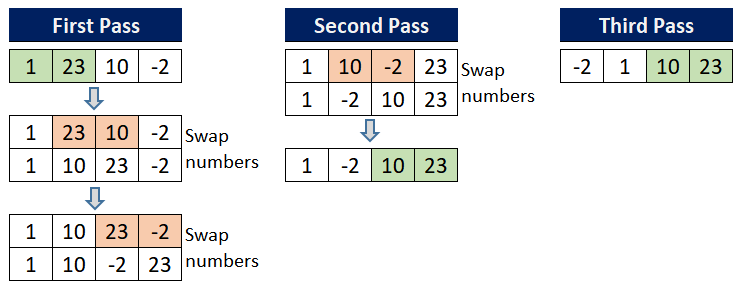
\includegraphics[width=105mm, height=40mm]{bubble_sort}} 
\end{figure}
\end{frame}

%%%%%%%%%%%%%%%%%%%%%%%%%%%%%%%%%%%%%%%%%%%%%%%%%%%%%%%%%%%%%%%%%%%%%%%%%%%%%%%%%%%%%%%%%%%%%%%%%%
\begin{frame}
\frametitle{Простые сортировки}
\framesubtitle{План лекции}

\begin{enumerate}
  \setcounter{enumi}{-1}
  \item{План лекции}
  \item{Задача сортировки}
  \item{Простые квадратичные сортировки}
  \item{\textcolor{blue} {Специальные сортировки}}
\end{enumerate}
\end{frame}


%%%%%%%%%%%%%%%%%%%%%%%%%%%%%%%%%%%%%%%%%%%%%%%%%%%%%%%%%%%%%%%%%%%%%%%%%%%%%%%%%%%%%%%%%%%%%%%%%%
\begin{frame}
\frametitle{Специальные сортировки}
\framesubtitle{Сортировка ?}
\justifying
\textbf{Задача}:\newline
Дан массив, состоящий из 1000 целых чисел, каждое из которых находится в интервале [0, 100].\newline\newline Отсортируйте данный массив.
\end{frame}

%%%%%%%%%%%%%%%%%%%%%%%%%%%%%%%%%%%%%%%%%%%%%%%%%%%%%%%%%%%%%%%%%%%%%%%%%%%%%%%%%%%%%%%%%%%%%%%%%%
\begin{frame}
\frametitle{Специальные сортировки}
\framesubtitle{Сортировка подсчётом}
\justifying
\textbf{Задача}:\newline
Дан массив, состоящий из 1000 целых чисел, каждое из которых находится в интервале [0, 100]. Отсортируйте данный массив.\newline\newline
\textbf{Ответ}: Сортировка подсчётом (counting sort)
\begin{figure}
    \captionsetup[subfigure]{labelformat=empty}
    \centering
    \subfigure[{ \scriptsize Сортировка подсчётом, Источник - \href{}{-} }]{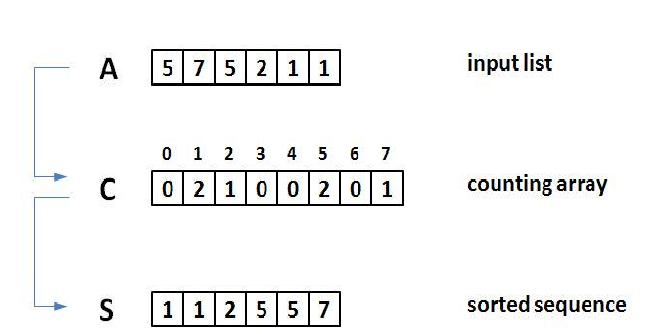
\includegraphics[width=80mm, height=40mm]{counting_sort}} 
\end{figure}
\end{frame}

%%%%%%%%%%%%%%%%%%%%%%%%%%%%%%%%%%%%%%%%%%%%%%%%%%%%%%%%%%%%%%%%%%%%%%%%%%%%%%%%%%%%%%%%%%%%%%%%%%
\begin{frame}
\frametitle{Специальные сортировки}
\framesubtitle{Блочная/карманная сортировка}
\justifying
\textcolor{red}{Блочная/карманная сортировка (bucket sort)}

Для карманной сортировки нужно разбить элементы массива входных данных на \textcolor{blue}{k} блоков (карманов, корзин). Далее каждый из таких блоков сортируется либо другой сортировкой, либо рекурсивно тем же методом разбиения. После сортировок внутри каждых блоков данные записываются в массив в порядке разбиения на блоки.\newline\newline
\textbf{Сложность:}\newline
Worst-case time complexity: $\mathcal{O}(n^2)$ \newline
Worst-case space complexity: $\mathcal{O}(n\cdot k$)\newline
\end{frame}

%%%%%%%%%%%%%%%%%%%%%%%%%%%%%%%%%%%%%%%%%%%%%%%%%%%%%%%%%%%%%%%%%%%%%%%%%%%%%%%%%%%%%%%%%%%%%%%%%%
\begin{frame}
\frametitle{Специальные сортировки}
\framesubtitle{Блочная/карманная сортировка}
\justifying
\textcolor{red}{Блочная/карманная сортировка (bucket sort)}
\begin{figure}
    \captionsetup[subfigure]{labelformat=empty}
    \centering
    \subfigure{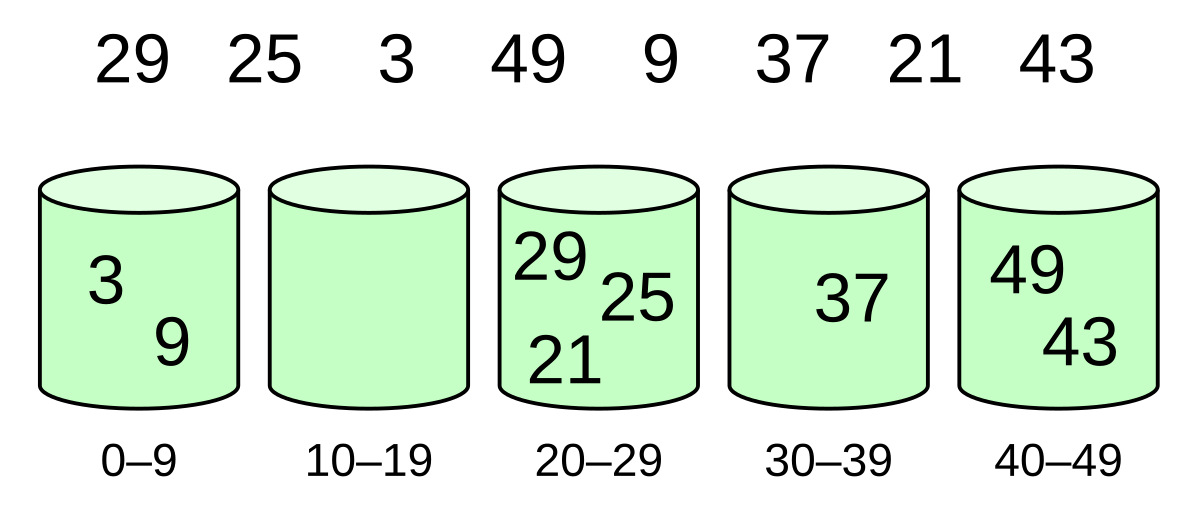
\includegraphics[width=65mm, height=27mm]{bucket_sort}}\newline
    \subfigure[{\scriptsize Сортировка подсчётом, Источник - \href{https://en.wikipedia.org/wiki/Bucket_sort}{Wikipedia} }]{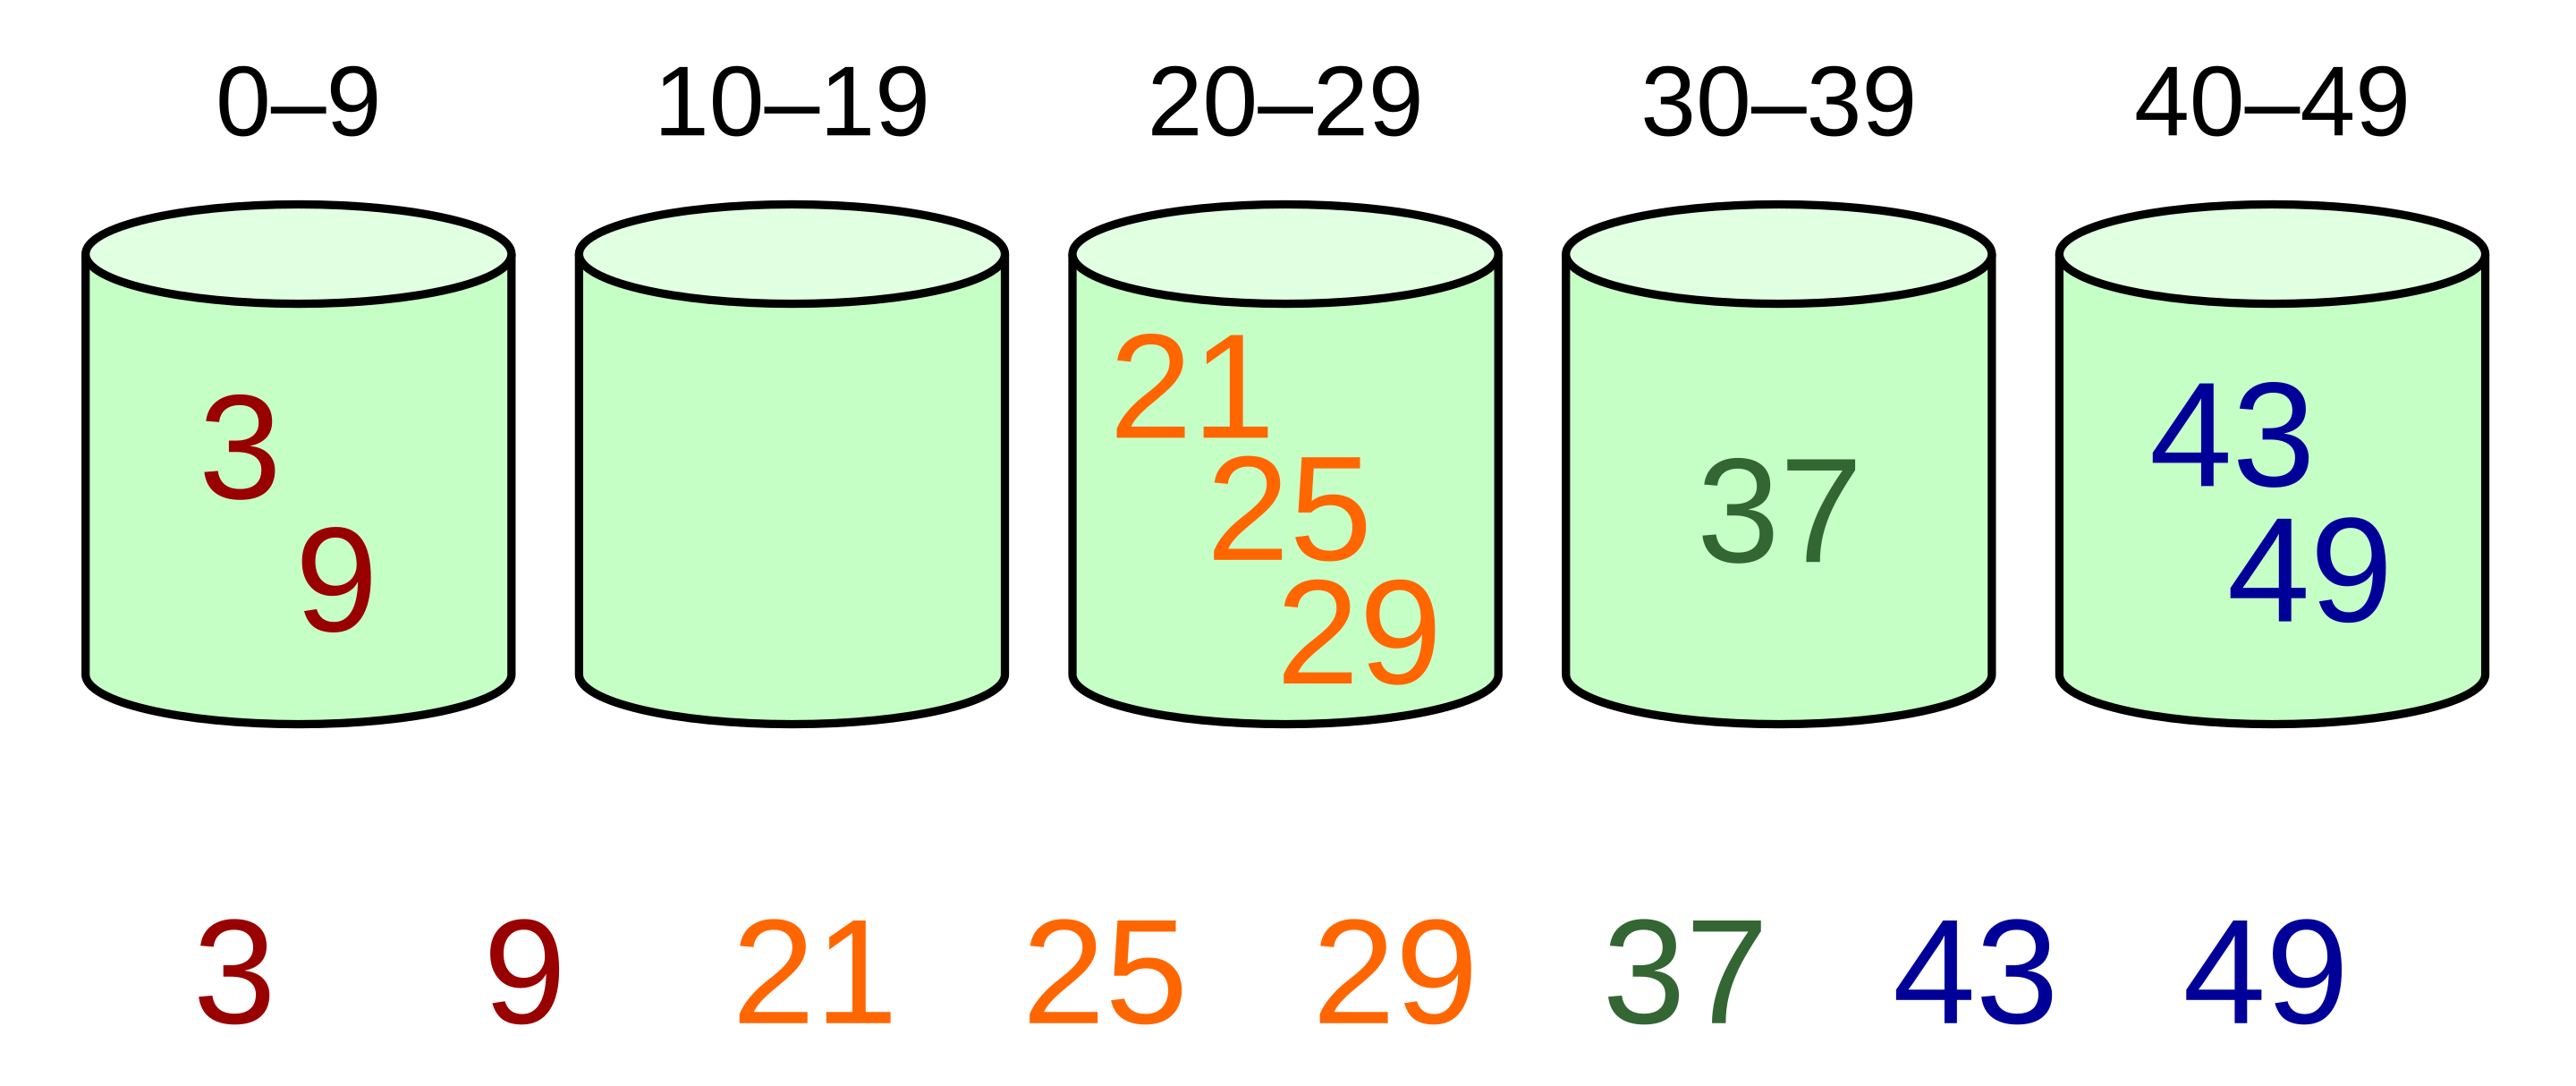
\includegraphics[width=65mm, height=27mm]{bucket_sort_2}}
\end{figure}
\end{frame}

%%%%%%%%%%%%%%%%%%%%%%%%%%%%%%%%%%%%%%%%%%%%%%%%%%%%%%%%%%%%%%%%%%%%%%%%%%%%%%%%%%%%%%%%%%%%%%%%%%
\begin{frame}
\frametitle{Специальные сортировки}
\framesubtitle{Блочная/карманная сортировка}
\justifying
\textcolor{red}{Блочная/карманная сортировка (bucket sort)}
\begin{figure}
    \captionsetup[subfigure]{labelformat=empty}
    \centering
    \subfigure[{\scriptsize Сортировка подсчётом, Источник - \href{https://neerc.ifmo.ru/wiki/index.php?title=Карманная_сортировка}{neerc.ifmo} }]{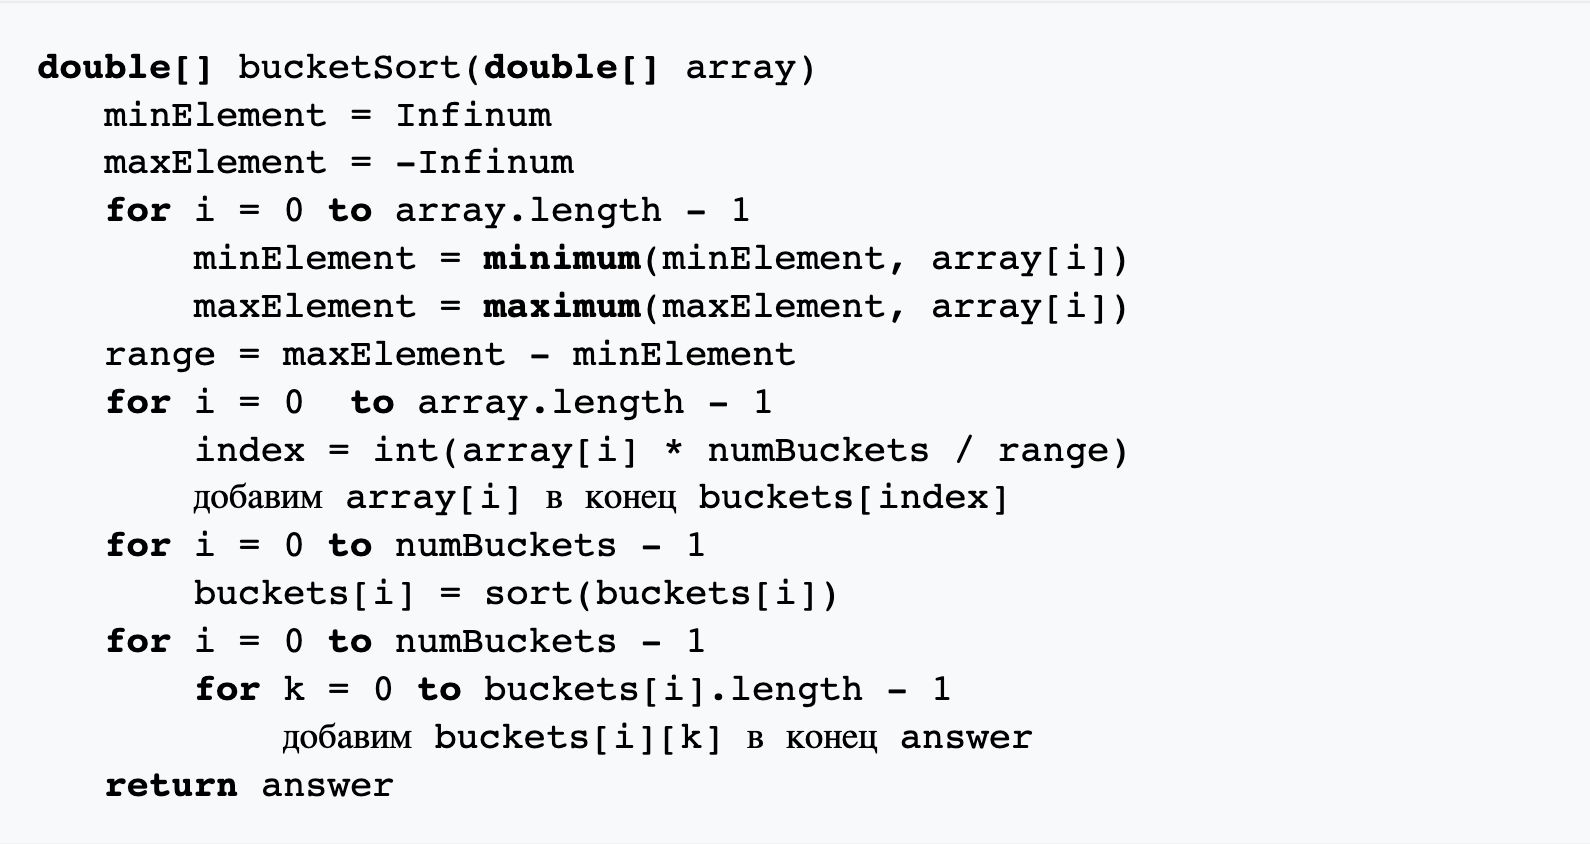
\includegraphics[width=95mm, height=55mm]{bucket_sort_pseudo}}
\end{figure}
\end{frame}

%%%%%%%%%%%%%%%%%%%%%%%%%%%%%%%%%%%%%%%%%%%%%%%%%%%%%%%%%%%%%%%%%%%%%%%%%%%%%%%%%%%%%%%%%%%%%%%%%%
\begin{frame}
\frametitle{Специальные сортировки}
\framesubtitle{Поразрядная сортировка}
\justifying
\textcolor{red}{Поразрядная сортировка (radix sort)}\newline
Разделение элементов массива на группы по их цифрам (разрядам) в определённой позиции и сортировка таких групп. Этот процесс повторяется для каждой позиции (разряда) числа, пока все элементы не будут упорядочены.\newline
\begin{figure}
    \captionsetup[subfigure]{labelformat=empty}
    \centering
    \subfigure[{\scriptsize Поразрядная сортировка, Источник - \href{https://brilliant.org/wiki/radix-sort/}{Brilliant.org} }]{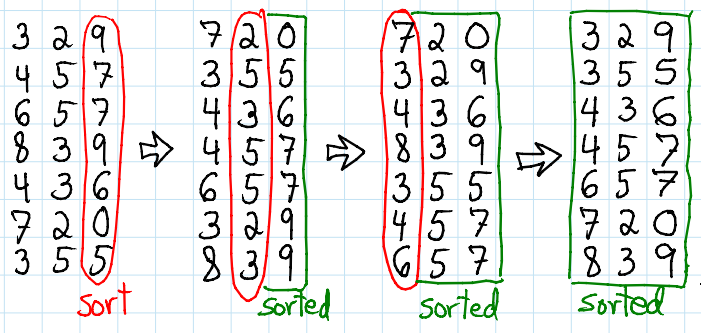
\includegraphics[width=95mm, height=40mm]{radix_sort}}
\end{figure}
\end{frame}

%%%%%%%%%%%%%%%%%%%%%%%%%%%%%%%%%%%%%%%%%%%%%%%%%%%%%%%%%%%%%%%%%%%%%%%%%%%%%%%%%%%%%%%%%%%%%%%%%%
\begin{frame}
\frametitle{Специальные сортировки}
\framesubtitle{Поразрядная сортировка}
\justifying
\textcolor{red}{Поразрядная сортировка (radix sort)}\newline
Сортировка по младшему разряду (для чисел)\newline
\begin{figure}
    \captionsetup[subfigure]{labelformat=empty}
    \centering
    \subfigure[{\scriptsize Поразрядная сортировка, Источник - \href{https://www.alphacodingskills.com/algo/radix-sort.php}{alphacodingskills} }]{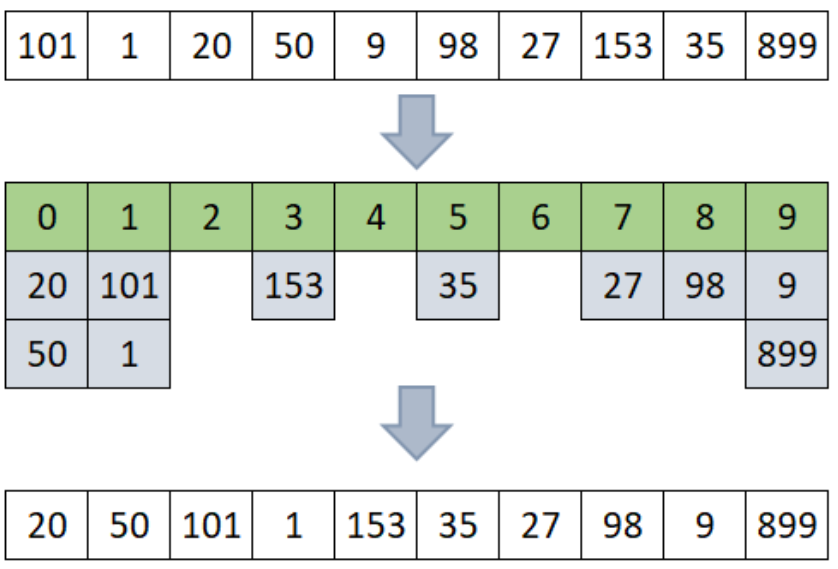
\includegraphics[width=75mm, height=50mm]{radix_sort_step1}}
\end{figure}
\end{frame}

%%%%%%%%%%%%%%%%%%%%%%%%%%%%%%%%%%%%%%%%%%%%%%%%%%%%%%%%%%%%%%%%%%%%%%%%%%%%%%%%%%%%%%%%%%%%%%%%%%
\begin{frame}
\frametitle{Специальные сортировки}
\framesubtitle{Поразрядная сортировка}
\justifying
\textcolor{red}{Поразрядная сортировка (radix sort)}\newline
Сортировка по разряду десятков\newline
\begin{figure}
    \captionsetup[subfigure]{labelformat=empty}
    \centering
    \subfigure[{\scriptsize Поразрядная сортировка, Источник - \href{https://www.alphacodingskills.com/algo/radix-sort.php}{alphacodingskills} }]{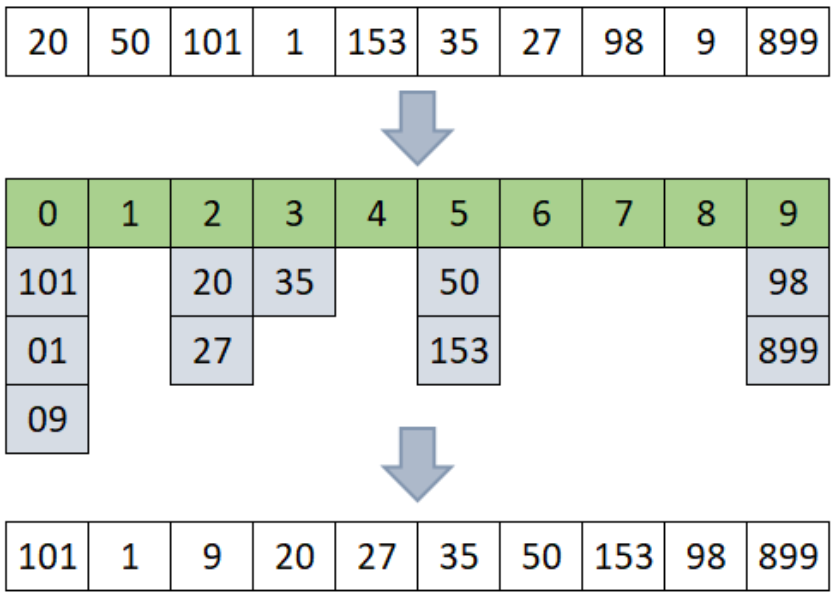
\includegraphics[width=75mm, height=50mm]{radix_sort_step2}}
\end{figure}
\end{frame}

%%%%%%%%%%%%%%%%%%%%%%%%%%%%%%%%%%%%%%%%%%%%%%%%%%%%%%%%%%%%%%%%%%%%%%%%%%%%%%%%%%%%%%%%%%%%%%%%%%
\begin{frame}
\frametitle{Специальные сортировки}
\framesubtitle{Поразрядная сортировка}
\justifying
\textcolor{red}{Поразрядная сортировка (radix sort)}\newline
Сортировка по старшему разряду
\begin{figure}
    \captionsetup[subfigure]{labelformat=empty}
    \centering
    \subfigure[{\scriptsize Поразрядная сортировка, Источник - \href{https://www.alphacodingskills.com/algo/radix-sort.php}{alphacodingskills} }]{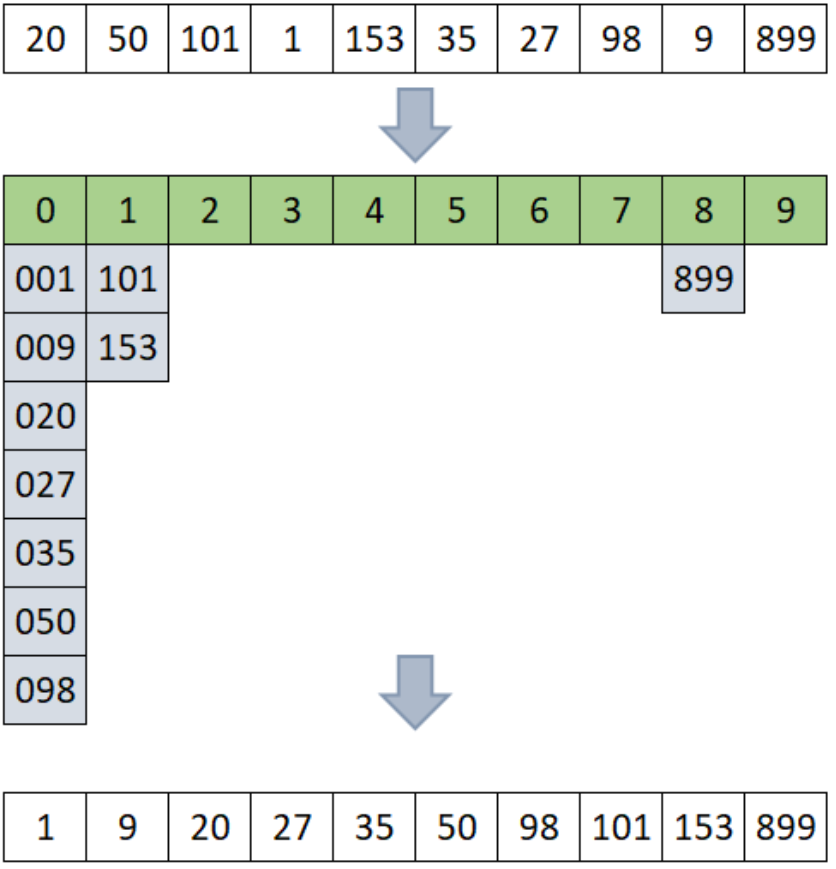
\includegraphics[width=60mm, height=49mm]{radix_sort_step3}}
\end{figure}
\end{frame}

%%%%%%%%%%%%%%%%%%%%%%%%%%%%%%%%%%%%%%%%%%%%%%%%%%%%%%%%%%%%%%%%%%%%%%%%%%%%%%%%%%%%%%%%%%%%%%%%%%
\begin{frame}
\frametitle{Специальные сортировки}
\framesubtitle{Поразрядная сортировка}
\justifying
\textcolor{red}{Поразрядная сортировка (radix sort)}\newline
Существует два варианта поразрядной сортировки:
\begin{itemize}
    \item{\textcolor{blue}{Least Significant Digit (LSD)} - от младшего разряда к старшему. Сначала идут более короткие элементы. Корректный порядок для чисел.\newline\newline Пример: [1, 2, 3, 4, 5, 6, 7, 8, 9, 10, 11]\newline}
    \item{\textcolor{blue}{Most Significant Digit (MSD)}- от старшего разряда к младшему. Лексикографический порядок. Подходит для сортировки строк.\newline\newline Пример: [1, 10, 2, 3, 4, 5, 6, 7, 8, 9]}
\end{itemize}
\end{frame}


\end{document}